%%% generic article type (pdf)latex file
%%% use together with Makefile

\documentclass[letterpaper]{scrartcl}
\usepackage{natbib}
\usepackage{graphicx}
\usepackage{amsmath,amsfonts,amsthm}
\usepackage{eufrak}
\usepackage{mathabx}
\usepackage{url}
\usepackage{framed}
\usepackage[usenames,dvipsnames,svgnames,table]{xcolor}
\usepackage[colorlinks]{hyperref}
\hypersetup{
     colorlinks   = true,
     urlcolor     = blue,
     linkcolor    = red,
     citecolor    = black
}
\usepackage{enumitem}
\usepackage{booktabs}
\usepackage{cprotect}
\usepackage{minted}

%\usepackage{wrapfig}
%\usepackage{subfig}
\usepackage[format=plain,labelsep=period,font=small,labelfont=bf]{caption}

%------------------------------------------------------------
% assignment
%
\newcommand{\anumber}{2}
%
%------------------------------------------------------------

% hyperref https://en.wikibooks.org/wiki/LaTeX/Hyperlinks#.5Chref
\urlstyle{same}

%% not working yet...
\newcounter{TotalPoints}
\newcounter{TotalBonus}

\newcommand{\BONUS}{\textsc{Bonus: }}
\newcommand{\bonus}[1]{\textbf{[bonus +#1*]}\stepcounter{TotalBonus}}
\newcommand{\points}[1]{\textbf{[#1 points]}\stepcounter{TotalPoints}}
\newenvironment{enuma}{\begin{enumerate}[label=(\alph*)]}{\end{enumerate}}
\newenvironment{enumi}{\begin{enumerate}[label=(\roman*)]}{\end{enumerate}}
\newenvironment{solution}{\par\noindent\P{} }{\ \qedsymbol}

\renewcommand{\vec}[1]{\ensuremath{\mathbf{#1}}}
\newcommand{\pd}[3][]{\left(\frac{\partial #2}{\partial #3}\right)_{#1}}

\newcommand{\anum}{0\anumber}

\title{{\Large Project \anumber: Planet watching in the TRAPPIST-1 System}}

\author{{\sffamily\large Project \emph{Comp. Methods Physics} ASU
    PHY494 (2017)}%
  \thanks{Current version of this document: \today. See
    Appendix~\protect\ref{sec:history} for a list of changes since v1
    from March 13, 2017.}}

\date{{\sffamily\large March 13, 2017 -- March 30, 2017}}


\begin{document}
\maketitle

\paragraph{Abstract}

Recently it was discovered that multiple planets orbit the ultracool
dwarf star TRAPPIST-1 about 40 light years from earth. All of these
planets are of a size comparable to earth and three orbit in the
habitable zone of their star and are therefore possible candidates for
worlds with liquid water and possibly life. Their very tight orbits
bring the planets into close vicinity.  It should be possible for an
observer to stand on one and to see multiple other planets in the
night sky so close nearby that continents would be easily discernible
with the naked eye.
%
Your task is to \emph{(1) simulate the innermost six planets of TRAPPIST-1}
and \emph{(2) analyze the visibility of nearby planets and to decide, which
of these planets would be the best one to visit for planet watching}. 
%
You will write a \emph{short report} to communicate, discuss and
summarize your reasoning and your results. The work is carried out in
teams of two or three students.

\begin{framed}
  \noindent
  Due Thursday, March 30, 2017, 11:59pm.
  \begin{itemize}
  \item Students work in teams of two or three students.
  \item \textbf{Admissible Collaboration:} Students are allowed to
    talk to other students in the class about the project and exchange
    ideas and tips. However, sharing/copying reports or full code
    solutions is not allowed. \textbf{Help from other students must be
      acknowledged in an Acknowledgments section}.  Direct help from
    outside the class is not allowed (except instructor/TA), e.g., you
    cannot ask for solutions (online or in person) but you can use
    books and resources on the internet to solve
    problems. \textbf{Cite all sources}. Code from the class can be
    used without explicit citation or acknowledgement.
  \item Each team should commit their  report (see
    Section~\ref{sec:report}) in \textbf{PDF} format to the team's
    \textbf{GitHub repository}; alternatively, combining report and
    code in a Jupyter notebook is also possible as long as the
    notebook can be read like a report (i.e., not just bullet points
    or short comments). If possible, also generate a PDF from your
    notebook and commit it together with everything else.
  \item The report \emph{must} contain a section
    \textbf{Contributions} at the end where the contributions of all
    team members are summarized. 
  \item Each team should commit and push \textbf{all code} (see
    Section \ref{sec:code}) that is required to reproduce the results
    in the report to their \textbf{GitHub repository}. Include a
    text file \textbf{\texttt{README.txt}} that describes the commands
    to run calculations. The code must run in the standard
    anaconda-based environment used for the class. If it is a Jupyter
    notebook then it should be possible to \emph{Kernel $\rightarrow$
      Restart \& Run All} and to produce all the required figures and
    output.
  \end{itemize}
  Grading will take the following into consideration:
  \begin{itemize}
  \item The code runs and produces correct output.
  \item The report clearly and succinctly describes the question,
    approach, and results and contains sufficient evidence that the
    requirements (see below) have been met.
  \item All team members contributed to the work: assessed by (1)
    Contributions section in the report, (2) commit history of the
    repository and comments in code, (3) short oral examination of
    team members (at instructor's discretion if deemed necessary).
  \item Code from outside sources (see Admissible Collaboration) and
    help is thoroughly attributed (Acknowledgements and References).
  \item \BONUS Additional work that you want to include in an appendix to
    the report or additional simulations for the main report will be
    treated as bonus material and can be awarded bonus points.
  \item \BONUS Elegant and fast code can be awarded bonus points.
  \end{itemize}
\end{framed}

\section{Submission instructions}

\noindent
%  \url{}
\fbox{\parbox{\linewidth}{Submission is to your private \textbf{team
      GitHub repository}. Follow the link provided to you by the
    instructor in order for the repository to be set up: It will have
    the name
    \emph{ASU-CompMethodsPhysics-PHY494/project-2-2017-\emph{YourTeamName}}
    and will only be visible your team and the instructor/TA. Follow the
    instructions below to submit this project.}}
Read the following instructions carefully. Ask if anything is unclear.
\begin{enumerate}
\item \texttt{git clone} your project repository (change
  \emph{YourTeamName} to your team's name)
  \begin{minted}[autogobble]{bash}
    repo="project-2-2017-YourTeamName.git" 
    git clone https://github.com/ASU-CompMethodsPhysics-PHY494/${repo}
  \end{minted}
  %$
  or, if you already have done so, \mintinline{bash}{git pull} from
  within your assignments directory.
\item  Create three sub-directories \texttt{Submission},
  \texttt{Grade}, and
  \texttt{Work}.
\item You can try out code in the \texttt{Work}
  directory but you don't have to use it if you don't want to. Your
  grade with comments will appear in
  \texttt{Grade}.
\item Create your solution in
  \texttt{Submission}. Use Git to \texttt{git
    add} files and \texttt{git commit} changes.

  You can create a PDF file or Jupyter notebook inside the
  \texttt{Submission} directory as well as Python
  code (if required). \textbf{Name your files \texttt{project\anum.pdf} or
    or \texttt{project\anum.ipynb}}, depending on how
  you format your work. Files with code (if requested) should be named
  exactly as required in the assignment.
\item When you are ready to submit your solution, do a final
  \texttt{git status} to check that you haven't forgotten anything,
  commit any uncommitted changes, and \texttt{git push} to your GitHub
  repository. Check on \emph{your} GitHub repository web
  page\footnote{\texttt{https://github.com/ASU-CompMethodsPhysics-PHY494/project-2-2017-\emph{YourTeamName}}}
  that your files were properly submitted.

  You can push more updates up until the deadline. Changes after the
  deadline will not be taken into account for grading.
\end{enumerate}
Work must be legible and intelligible or may otherwise be
returned ungraded with 0 points.

\section{Problem description}
\label{sec:problem}

Recently, at least seven earth-sized exoplanets were discovered
orbiting the ultracool dwarf star TRAPPIST-1, about 40 light years
away from earth \citep{Gillon:2016aa, Gillon:2017aa}. Using transit
measurements of the planets in front of their host star using the
Spitzer space telescope and ground-based instruments, orbital
parameters for six of these planets (named TRAPPIST-1b to TRAPPIST-1g)
could be determined.\footnote{A seventh planet, TRAPPIST-1h, was
  observed but no orbital parameters could be determined. TRAPPIST-1h
  will be ignored in this problem.} The planets orbit very close to
TRAPPIST-1, at distances between $11\times 10^{-3}$~au (astronomical
units, average distance earth-sun\footnote{1~au is defined to be
  149,597,870.700~km.}) to about $45\times 10^{-3}$~au
\citep{Gillon:2017aa}. TRAPPIST-1 is very cool (effective temperature
2600~K) and small (0.0802 of the solar masses, 0.117 of the solar
radius) and hence even in these small orbits at least three planets
(TRAPPIST-1e, TRAPPIST-1f, and TRAPPIST-1g) are predicted to be in the
habitable zone where liquid water could exist.

This discovery has spurred the imagination, with people wondering what
it would be like to be on these planets (Figure~\ref{fig:poster}). In
particular, the close vicinity of the planets would make it possible
to see multiple other planets in the sky. Some of these planets might
come so close that one could, in principle, be able to see continents
or even smaller landmarks and structures with the naked eye.

\begin{figure}[btp]
  \centering
  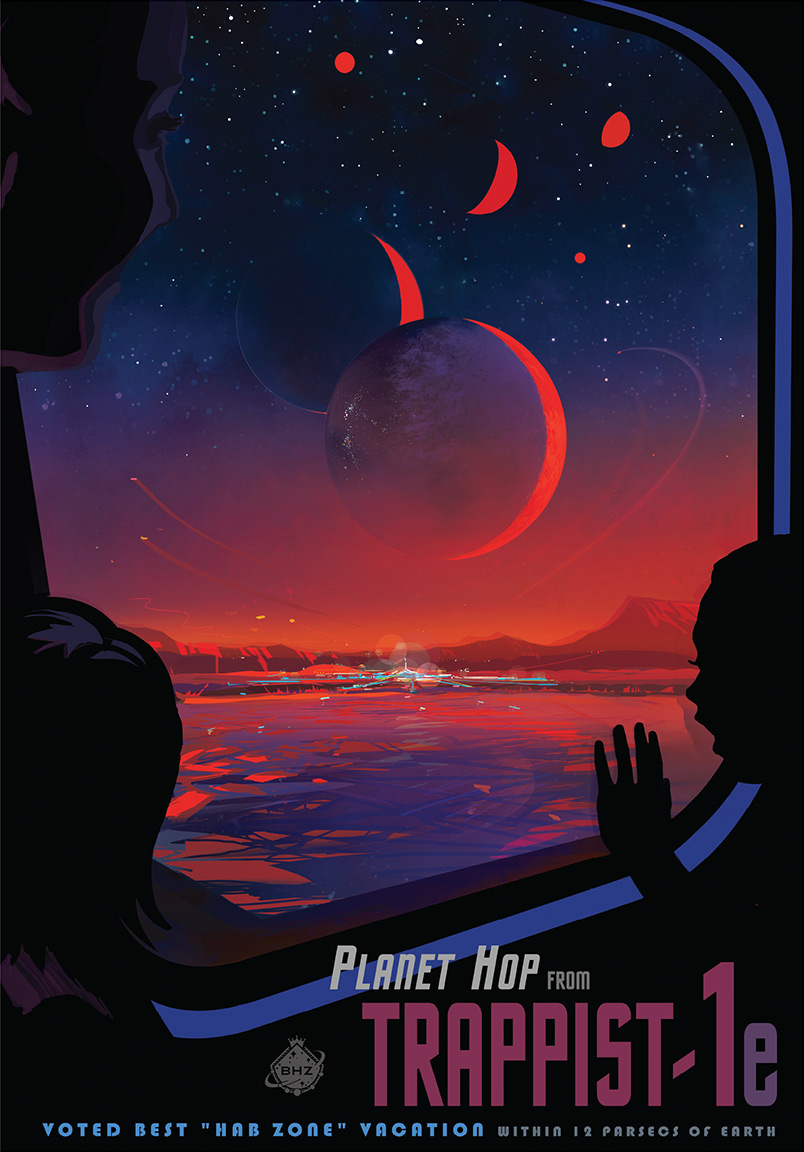
\includegraphics[height=0.88\textheight]{figs/2159_posternormalsize.jpg}
  \caption{A poster advertising space tourism in the TRAPPIST-1 system. It
    shows a hypothetical view from TRAPPIST-1e with six other planets
    (b, c, d, f, g, and h) visible in the sky. (Copyright \copyright 2017
    NASA, from
    \href{https://exoplanets.nasa.gov/resources/2159/?linkId=34784370}{NASA
      Exoplanet Exploration: Galleries: TRAPPIST-1}).}
  \label{fig:poster}
\end{figure}

In this work you will be simulating the TRAPPIST-1 system and analyze
the trajectories of the planets to find out which planet offers the
best view on nearby other planets. In particular, use your simulations
to decide if the poster in Figure~\ref{fig:poster} is scientifically
accurate: \emph{Will someone on TRAPPIST-1e be able to see five other
  planets in the sky so that details of their surfaces would in
  principle be visible with the naked eye?}\footnote{The poster shows
  \emph{six} planets but we are ignoring TRAPPIST-1h (which would be
  the smallest planet in the poster) in this project because we do not
  have enough data to simulate it.}


\subsection{TRAPPIST-1 system}
\label{sec:system}

Consider the following for your orbital simulation of the TRAPPIST-1 system.

\paragraph{Interactions}

The planets interact with the central star and with each other through
Newton's law of gravitation.

\paragraph{Parameters and constants}

Use the orbital parameters from Table 1 in \citet{Gillon:2017aa} (as
provided in file \texttt{parameters.py} in the dictionaries
\texttt{parameters.planets} and \texttt{parameters.star}) to simulate
the TRAPPIST-1 system with the six innermost planets, b--g.

If you use the parameters as given in \texttt{parameters.planets} then
the units for the planets are as follows: mass $m$ in multiples of the
star's mass, orbital semi-major axis $a$ in $10^{-3}$~au and
eccentricity as unit-less number, orbital period $P$ in days; the
planetary radius $R$ is given in earth radii. The mass of TRAPPIST-1
in these units is 1. Importantly, the gravitational constant in these
units is
\begin{gather}
  \label{eq:G}
  G = 4\pi^{2} \times 0.0802 \times \frac{(10^{3})^{3}}{364.25^{2}}.
\end{gather}
(and is available as \texttt{parameters.G\_local}). For other
constants see the file \texttt{parameters.py}.


\paragraph{Initial conditions}

The planets move on elliptical orbits with the star at one focus; the
ellipses are defined by their major axes $a$ and eccentricities
$e$. All planets move in the same plane. The following Keplerian
equations determine their \emph{initial conditions} at aphelion:
$r_\text{max}$ is the distance of the star to the aphelion (farthest)
point of orbit; $r_\text{min}$ to perihelion:
\begin{gather}
  r_\text{max} = a(1+e)\label{eq:aphelion}\\
  r_\text{min} = a(1-e)\label{eq:perihelion}
\end{gather}
The velocity $v_\text{ap}$ at the aphelion is
\begin{gather}
  \label{eq:vap}  
  v_\text{ap} = \sqrt{\frac{GM}{a} \frac{1-e}{1+e}}
\end{gather}
with $M$ the mass of the star and the velocity vector $\vec{v}$ is
perpendicular to the radial vector.

For simplicity, assume that at $t=0$ all planets are at their
respective aphelion (i.e., all planets are on a line on the same side
of their star).\footnote{This assumption is somewhat justified by
  the observation that the ratios of periods of the planets are all
  close to ratios of small integers and hence a full conjunction will
  occur eventually. Such a resonance suggests that all planets formed
  farther out together and then migrated inwards
  \citep{Gillon:2017aa}.}

\paragraph{Motion of the central star}

You may assume that the central star is fixed at the center of the
coordinate system, which is based on the observation that the star's
mass is much larger than the planet masses, $M_{\text{star}} \gg
m_{\text{planet}}$. 

For a \BONUS project (see below) you should relax this assumption and
treat the central star as just another body in the
simulation. However, in this case you should choose your \emph{initial
  conditions} such that the \emph{total momentum} of the whole system
$\vec{P = M_{\text{star}}\vec{v}_{\text{star}} + \sum_{i=1}^{6}m_{i}
  \vec{v}_{i}}$
is 0, corresponding to the center of mass of the system at rest. This
is most easily accomplished by setting $\vec{v}_{\text{star}}$ so that
$\vec{P}=0$.

\subsection{Analysis of accuracy}
\label{sec:accuracy}

We want to assess the accuracy of the orbital simulations. You should
perform at least the following two tests (see also the Objectives in
\ref{sec:tasks}).

\subsubsection{Orbital period}
\label{sec:period}

Test that the simulation reproduces the observed orbital periods (see
values in Table 1 in \citep{Gillon:2017aa}).

\subsubsection{Energy conservation}
\label{sec:energy}

Newton's equations of motion for time- and velocity-independent
potentials conserve the total energy. Test that the total energy of
the system
\begin{gather}
  \label{eq:energy}
  E = T + U
\end{gather}
is conserved, $dE/dt = 0$. $T$ is the kinetic energy and $U$ is the
potential energy of the system
\begin{align}
  \label{eq:KE}
  T &= \frac{1}{2} \sum_{i=1}^{N} m_{i} \vec{v}_{i}^{2}\\
  \label{eq:PE}
  U &= \frac{1}{2}\sum_{i=1}^{N}\sum_{\substack{j=1\\j \neq i}}^{N} U_{ij}.
\end{align}

Plot the base-10 logarithm of relative error in the total energy 
\begin{gather}
  \label{eq:energyaccuracy}
  \epsilon(t) = \log_{10} \frac{E(t) - E(t=0)}{E(t=0)} 
\end{gather}
to estimate the accuracy of your integration scheme.\footnote{See
  \texttt{integrators2.py} from class
  \emph{\href{http://asu-compmethodsphysics-phy494.github.io/ASU-PHY494//2017/02/16/11_ODEs/}{11
      ODEs}} for code that you can adapt for this purpose.}

\subsubsection{BONUS: Momentum conservation}
\label{sec:momentum}

\BONUS If you are also simulating the system with the central star
moving freely you know that the center of mass of the total system is
initially at rest and thus the total momentum $\vec{P}=0$. No external
forces are at work so the total momentum cannot change,
$d\vec{P}/dt = 0$ and hence the total momentum ought to be zero for
\emph{all} time steps. Test that in your simulation the total momentum
fulfills $\vec{P} = 0$ for all time steps.


\subsection{Analysis of ``nearby'' planets}
\label{sec:nearby}

We want to estimate how many \emph{nearby} planets can be seen from
each of the planets in the system at any point in time. From this time
series of counts for each planet we can then calculate probabilities
$P_{i}(\nu)$ for seeing $\nu$ nearby planets\footnote{$\nu$ is the
  greek letter ``nu'' and not lower-case V.}, assuming the observer is
located on planet $i$.\footnote{As a simplifying assumption, we only
  consider distances between planets and do not consider where on the
  planet surface the observer would be located. You are more than
  welcome to extend the project in this direction for additional bonus
  points.}

\paragraph{Definition of \emph{nearby planets}}

We define \emph{nearby} to mean \emph{within a distance $d_{0}$ so
  that features of size 1000 km or greater can be distinguished with
  the naked eye.}

\paragraph{Resolution of the naked eye}

The naked eye can typically resolve two different objects if they are
at least one arc minute apart\footnote{One arc minute is 1/60 of a
  degree: $1' = \frac{1}{60}^{\circ}$}, i.e., its resolution is
\begin{gather}
  \label{eq:thetaeye}
  \theta_{\text{eye}} = 1'
\end{gather}
The condition for resolving an object by naked eye is that the object
has to appear under an angular separation 
\begin{gather}
  \label{eq:resolution}
  \alpha \ge \theta_{\text{eye}}.
\end{gather}
The viewing angle $\alpha$ can be computed from the size of the object
$y$ (its actual separation) and its distance $d$ from the
observer. This allows one to find a maximum distance
$d_{0} = d(y_{\text{min}})$ so that features of size
$y_{\text{min}} = 1000\,\text{km}$ can still be resolved. A
\emph{nearby planet} is then a planet within a distance $d \le d_{0}$.


\section{Report}
\label{sec:report}

Write a report in which you address the objectives in Section
\ref{sec:tasks} below in the context of the problem (Section
\ref{sec:problem}). The report should contain all results (figures,
tables, equations). It must contain a \emph{title}, \emph{author's
  name}, sections \emph{Background} (problem description, definitions,
any equations that you use), \emph{Results and Discussion}
(description and interpretation of results), and \emph{Summary} (short
summary of the main results).

The report \emph{must} contain a section \emph{Contributions} where
you summarize the contributions of each team member. For example, for
a team consisting of three members with initials A.B., C.D.E., and
F.G., the beginning of this section could be written along the lines
of
\begin{quotation}
  A.B.\ wrote the code to initialize the planet positions and
  velocities with help from C.D.E. C.D.E.\ wrote the integration
  routine, A.B., C.D.E., and F.G. together wrote the simulation
  function \texttt{orbit()}. F.G.\ with help from A.B.\ wrote the
  orbit plotting code and produced figures 1 and 2. F.G.\ also wrote
  the Background section \dots
\end{quotation}
(Note that all team members should have commits in the team
reporsitory.)

If you had any form of outside help you must describe it in an
\emph{Acknowledgments} section. 

If you use code or material from elsewhere you \emph{must cite the
  source} (add a \emph{References} section). 

Any bonus material can be shown in an optional \emph{Appendix}.

The report must be written in full sentences and read as a coherent
piece of work. Figures must have legends, labels, and captions. Type
set in an 11pt font with single line spacing (captions, labels, legend
may have smaller font sizes but must still be legible) and leave at
least 1~in margins. 

Overall, a length of about four pages is expected for a written
document produced with a word processor; the report should
not be less than three or more than six pages long.

\section{Code}
\label{sec:code}

For all numerical calculations use Python 3.x. You may use any of the
Python packages that are part of the Anaconda 3 distribution such as
\texttt{numpy} and \texttt{matplotlib}. 

Include all the code that is needed to generate the results shown in
your report. This can consist of Python programs, modules, a Jupyter
notebook, or a mixture thereof. Include a separate file
\texttt{README.txt} that explains how to run your code in order to
generate the results in your report. Your code must run in order for
you to be awarded full marks.


\section{Objectives}
\label{sec:tasks}
Address the following objectives in your report while taking all
requirements in Section \ref{sec:problem} into account:
\begin{enuma}
\item Simulate the TRAPPIST-1 system (star and planets b to g) by
  solving the Newtonian equations of motions using Python code. Your
  code should produce the positions and velocities of all planets for
  all time steps.
  \begin{enumi}
  \item Generate initial conditions for the six planets b to g.
  \item Plot the orbits for all six planets for a maximum time period
    of 1.5 d in the $x$-$y$ plane. Add a marker for the central star
    to your plot. Confirm that your result is consistent with the
    known period $P_{b}$ for planet TRAPPIST-1b (see also Section
    \ref{sec:period}).
  \item Plot the orbits for all six planets for a maximum time period
    of 1000 d in the $x$-$y$ plane. Add a marker for the central
    star.\footnote{\BONUS analyse the time series of the angular
      motions of the planets to show that their computed periods
      $P_{i}$ match the experimentally observed ones (see Section
      \protect\ref{sec:period}).} \emph{Use the trajectories from this
      run for further analysis.}
  \item Determine the accuracy of your integration algorithm by
    plotting as a function of time (1) the total energy $E(t)$
    together with kinetic energy $T$ and potential energy $U$
    (Eqn.~\ref{eq:energy}--\ref{eq:PE}) and (2) the logarithm of the
    relative error in the energy $\epsilon(t)$
    (Eq.~\ref{eq:energyaccuracy}).
  \end{enumi}
  Describe and justify your algorithm and your choices of parameters (e.g., your
  time step). Describe and discuss your figures.
\item \BONUS Treat the central star not as fixed but as another body
  in the simulation. 
  \begin{enumi}
  \item Plot the path of the star over 1000~d and compare the extent
    to the star's diameter. Is the center of mass of the whole system
    inside the star?
  \item Analyze the ``wobble'' of the star (motion due to gravity of
    the planets). Assume an observer looks side on the system along
    the $y$-direction. Compute a time series of the $y$-component of
    the velocity of the star $\vec{v}_{*}$ in the observer's frame of
    reference (transform from center-of-mass frame to lab frame of
    reference):
    \begin{gather}
      \label{eq:vstarlabframe}
      \vec{v}_{*} - \frac{\sum_{i=1}^{N_{\text{planets}}}
        m_{i}}{M_{\text{star}} + \sum_{i=1}^{N_{\text{planets}}} m_{i}}\vec{v}
    \end{gather}
    Compare the changes to the resolution of current Doppler
    spectrometers (about 1 m/s). Would the wobble be detectable?
  \end{enumi}
\item Using the positions of all planets $\vec{r}_{i}(t)$ for $0 \leq
  t \leq 1000\,\text{d}$, find the planets where an observer is most
  likely to see many other planets \emph{nearby} (as defined in Section
  \ref{sec:nearby}).
  \begin{enumi}    
  \item Given the resolution of the naked eye, Eq.~\ref{eq:thetaeye},
    determine the maximum distance $d_{0}$ for two planets so that an
    observer could still resolve large-scale landscape features of
    size $y = 1000\,\text{km}$.
  \item Analyze $\vec{r}_{i}(t)$ to find for each time step the number
    of planets $\nu_{i}(t)$ that are nearby to planet $i$ (excluding
    the planet itself). Plot $\nu_{i}(t)$ for $i=4$ (TRAPPIST-1e) (and
    other planets if necessary for your discussion).
  \item For each planet $i$, calculate the probability over the 1000 d
    observation time to have exactly $\nu$ other planets nearby,
    $P_{i}(\nu)$.\footnote{You may perform these calculations in any
      way that you like. You might, however, find it useful to look at
      the NumPy \texttt{numpy.histogram()} and/or Matplotlib
      \texttt{matplotlib.pyplot.hist()} functions.} 
    
    Plot the probabilities $P_{i}(\nu)$ for all six planets. 
  \end{enumi}
\item Using your results, answer the question if the poster in
  Figure~\ref{fig:poster} is scientifically accurate: \emph{Will
    someone on TRAPPIST-1e be able to see five other planets in the
    sky so that details of their surfaces would in principle be
    visible with the naked eye?}

  Which would be the best planets in the TRAPPIST-1 system for
  ``planet watching''?
\end{enuma}

\section{History}
\label{sec:history}

Changes and updates to this document.
\begin{description}
\item[2017-03-13] initial version
\item[2017-03-13] updated: accuracy analysis added
\item[2017-03-16] fixed $G$ (Eq.~\ref{eq:G}) but note
  \texttt{parameters.G\_local} was correct; corrected wobble velocity
  (new Eq.~\ref{eq:vstarlabframe}) in bonus problem
\end{description}

\bibliographystyle{physbiol-natbib}      % basic style, author-year citations
\bibliography{phy494}   % name your BibTeX data base

\end{document}

%%% Local Variables: 
%%% mode: latex
%%% TeX-master: t
%%% End: 
